%% LaTeX2e class for student theses
%% thesis.tex
%% 
%% Karlsruhe Institute of Technology
%% Institute for Program Structures and Data Organization
%% Chair for Software Design and Quality (SDQ)
%%
%% Dr.-Ing. Erik Burger
%% burger@kit.edu
%%
%% See https://sdq.kastel.kit.edu/wiki/Dokumentvorlagen
%%
%% Version 1.3.6, 2022-09-28

%% Available page modes: oneside, twoside
%% Available languages: english, ngerman
%% Available modes: draft, final (see README)
\documentclass[twoside, ngerman]{sdqthesis}

%% ---------------------------------
%% | Information about the thesis  |
%% ---------------------------------

%% Name of the author
\author{Simon Ding}

%% Title (and possibly subtitle) of the thesis
\title{Automatisierung von GUI-Tests für Webanwendungen durch den Einsatz großer Sprachmodelle}

%% Type of the thesis 
\thesistype{Masterarbeit}

%% Change the institute here, ``KASTEL'' is default
% \myinstitute{Institute for \dots}

%% You can put a logo in the ``logos'' directory and include it here
%% instead of the SDQ logo
% \grouplogo{myfile}
%% Alternatively, you can disable the group logo
% \nogrouplogo

%% The reviewers are the professors that grade your thesis
\reviewerone{Prof. Dr.-Ing. Anne Koziolek}
\reviewertwo{Prof. Dr. Ralf Reussner}

%% The advisors are PhDs or Postdocs
\advisorone{Dipl.-Ing. Daniel Zimmermann}
%% The second advisor can be omitted
%\advisortwo{M.Sc. D}

%% Please enter the start and end time of your thesis
\editingtime{05. September 2023}{05. März 2024}

\settitle

%% --------------------------------
%% | Bibliography                 |
%% --------------------------------

%% Use biber instead of BibTeX, see README
\usepackage[citestyle=numeric,style=numeric,backend=biber]{biblatex}
\addbibresource{thesis.bib}

%% --------------------------------
%% | Packages                     |
%% --------------------------------
\usepackage{pgfgantt}

\usepackage[T1]{fontenc}
\usepackage{caption}
\usepackage{subcaption}
\usepackage{pgfplots}

\usepgfplotslibrary{fillbetween}


%% --------------------------------
%% | Custom Commands              |
%% --------------------------------
\newboolean{showtodos}
\setboolean{showtodos}{true}
\newcommand{\todo}[1]{\ifthenelse{\boolean{showtodos}}{\textcolor{red}{TODO: #1}}{}}

%% ====================================
%% ====================================
%% ||                                ||
%% || Beginning of the main document ||
%% ||                                ||
%% ====================================
%% ====================================
\begin{document}

%% Set PDF metadata
\setpdf

%% Set the title
\maketitle

%% The Preamble begins here
\frontmatter

\input{sections/declaration.tex}

\setcounter{page}{1}
\pagenumbering{roman}

%% ----------------
%% |   Abstract   |
%% ----------------
 
%% For theses written in English, an abstract both in English
%% and German is mandatory.
%%
%% For theses written in German, a German abstract is sufficient.
%%
%% The text is included from the following files:
%% - sections/abstract

\includeabstract

%% ------------------------
%% |   Table of Contents  |
%% ------------------------
\tableofcontents

%\listoffigures
%\listoftables

%% -----------------
%% |   Main part   |
%% -----------------

\mainmatter

%% LaTeX2e class for student theses
%% sections/content.tex
%% 
%% Karlsruhe Institute of Technology
%% Institute for Program Structures and Data Organization
%% Chair for Software Design and Quality (SDQ)
%%
%% Dr.-Ing. Erik Burger
%% burger@kit.edu
%%
%% Version 1.3.6, 2022-09-28

\chapter{Einleitung}
\label{ch:Introduction}

% testen ist wichtig

Das Testen von Software ist ein wichtiger Bestandteil der Softwareentwicklung, der sicherstellt, dass die Software wie erwartet funktioniert und die festgelegten Anforderungen erfüllt.
Es gibt verschiedene Arten von Softwaretests, darunter Unit-Tests, Systemtests und Akzeptanztests \cite{Sommerville10}.
Im Folgenden wird der Fokus auf funktionale Systemtests von Webanwendungen gelegt, die die gesamte Anwendung testen und dabei als Blackbox betrachten \cite{Beizer1990}.
Diese werden in Kapitel \ref{sec:Foundations:GUIBasedSystemTests} näher beschrieben.

% testen speziell von GUIs ist wichtig

Zumindest einzelne Komponenten einer Webanwendung werden gewöhnlich in dem Webbrowser des Benutzers ausgeführt, in dem die Anwendung auch dargestellt wird.
Dadurch ergeben sich besondere Herausforderungen für das Testen von Webanwendungen.
Einerseits verschärfen die Ausführung von Anwendungscode und Darstellung im Browser das Problem der Flakiness, bei der Tests kein konsistentes Ergebnis liefern, auch wenn die Anwendung nicht geändert wurde.
Gleichzeitig bedeuten Änderungen an der grafischen Benutzeroberfläche (Englisch: graphical user interface, GUI) oft, dass auch die Tests geändert werden müssen \cite{ChallengesSelenium}.
Lösungsansätze für diese Probleme sind Gegenstand aktiver Forschung und eine Auswahl wird in Kapitel \ref{ch:RelatedWork} vorgestellt.

% es wäre schön, wenn Tests ohne hartkodierte Fehlerbedingungen Fehler erkennen könnten

Diese Arbeit schließt an die Arbeit von \Citeauthor{GPT3Testing} an.
Ihr Ansatz ermöglicht das automatische Testen über GUIs, was sie an einer einfachen Webanwendung evaluieren.
Sie verwenden ein großes Sprachmodell (Englisch: large language model, LLM), um Benutzerinteraktionen zu generieren, mit denen die Anwendung getestet wird.
Dabei handelt es sich um eine Anwendung aus dem Bereich des maschinellen Lernens, die in der Lage ist, kontextuell angemessene Antworten auf eine Vielzahl von Aufgaben zu generieren \cite{FewShotLearners}.
Das LLM bekommt eine strukturierte Repräsentation der grafischen Benutzeroberfläche, vorherige Benutzerinteraktionen und eine natürlichsprachliche Testbeschreibung als Eingabe.
Es wird aufgefordert, eine Benutzerinteraktion zu generieren, die anschließend automatisch in der Anwendung ausgeführt wird \cite{GPT3Testing}.

In den Kapiteln \ref{ch:ExperimentalSetup} und \ref{ch:Results} liefert diese Arbeit zwei Beiträge:
Erstens wird der Ansatz an einer komplexeren Webanwendung mit verschiedenen Möglichkeiten zur Interaktion getestet.
Zweitens wird untersucht, ob das LLM gleichzeitig als Testorakel verwendet werden kann, das heißt, ob das LLM auch in der Lage ist, Fehlerzustände zu erkennen.

Absatz über \ref{ch:Conclusion}

Zuletzt befindet sich in Anlage \ref{ch:PracticalNotes} eine Sammlung von Erkenntnissen, die sich im Verlauf dieser Arbeit gezeigt haben und die für den praktischen Einsatz hilfreich sein könnten.


% LLMs sind vielversprechend \cite{GPT3Testing}, 

\chapter{Grundlagen}
\label{ch:Foundations}

\section{Systemtests auf Grundlage von grafischen Benutzeroberflächen}
\label{sec:Foundations:GUIBasedSystemTests}
Softwaretests sind ein wesentlicher Bestandteil der Softwareentwicklung.
Er umfasst die Bewertung einer Softwareanwendung oder eines Systems, um etwaige Mängel oder Fehler zu erkennen, die die Funktionalität, Zuverlässigkeit oder Leistung beeinträchtigen könnten.
Das Ziel von Softwaretests ist es, sicherzustellen, dass die Software wie erwartet funktioniert und die festgelegten Anforderungen erfüllt.
Es gibt verschiedene Arten von Softwaretests, darunter Unit-Tests, Integrations-Tests, Systemtests und Akzeptanztests.
Das Testen eines GUI-basierten Systems, bei dem nur auf die GUI zugegriffen wird, nennen wir einen GUI-basierten Systemtest oder GUI-Test.
Es wird oft von Software-Testern oder Qualitätssicherungsexperten durchgeführt, die eine Kombination aus manuellen und automatisierten Testmethoden benutzen, um Fehler zu erkennen und sicherzustellen, dass die Software die gewünschten Qualitätsstandards erfüllt.
Manuelle Tests sind ein gängiger Ansatz für GUI-basierte Systemtests, bei denen Tester Testfälle manuell ausführen, Benutzeraktionen simulieren und Beobachtungen und Feedback aufzeichnen.
Es können auch automatisierte Testtools wie Selenium und Appium verwendet werden, um GUI-Tests zu automatisieren, wodurch die Effizienz und Genauigkeit des Testprozesses erhöht werden kann.

GUI-Tests können grob in exploratives Testen und Testen auf der Grundlage von Designer-Testfällen unterteilt werden.
Beim explorativen Testen besteht das Ziel in der Regel darin, Pfade in der zu testenden Anwendung (Englisch: application under test, AUT) zu finden, die zu Abstürzen führen.
Eine grundlegende Technik für exploratives Testen, die leicht automatisiert werden kann, ist das Monkey-Testing, bei dem zufällige Benutzeraktionen simuliert werden.
Im Gegensatz dazu sind Tests, die von Designern spezifiziert werden, oft sehr viel kostspieliger.
Um diese zu automatisieren, müssen die Programmierer aus der Spezifikation ein Testskripte ableiten, die parallel zu Änderungen an der grafischen Benutzeroberfläche gewartet werden müssen.
Dies ist ein Problem, da die grafische Benutzeroberfläche oft der sich am häufigsten ändernde Teil eines Systems ist.

\section{Transformer: Ein Überblick}
\label{subsec:Foundations:Transformer}
Transformer \cite{transformers} sind eine Klasse von Deep-Learning-Modellen, die sich bei einer Vielzahl von Aufgaben der Linguistischen Datenverarbeitung wie maschineller Übersetzung, Texterzeugung und Sprachmodellierung als äußerst effektiv erwiesen hat \cite{transformers,bert,FewShotLearners,gpt4}.
Sie basieren auf einer Architektur, die sich von herkömmlichen rekurrenten neuronalen Netzen (RNNs) und Convolutional Neural Networks (CNNs) unterscheidet.
In jedem Schritt der Verarbeitung wird die Eingabesequenz zu jeweils einem Ausgabetoken verarbeitet.
Durch wiederholte Anwendung kann so eine Sequenz von Ausgabetoken erzeugt werden.
Ein grundlegender Baustein eines Transformator-Modells ist der Self-Attention-Mechanismus, der es dem Modell ermöglicht, sich während der Kodierungs- und Dekodierungsphasen auf bestimmte Teile der Ein- und Ausgabesequenzen zu „konzentrieren“.
Er ist notwendig um Abhängigkeiten zwischen weit voneinander entfernten Teilen der Eingabe zu erfassen, was besonders wichtig für Aufgaben des Sprachverständnisses ist.
In einem Transformer-Modell wird die Eingabesequenz zunächst von einer Reihe von Kodierungsschichten verarbeitet, die jeweils aus einem Self-Attention-Modul und einem neuronalen Feedforward-Netzwerk bestehen.
Das Self-Attention-Modul berechnet eine Gewichtung der Aufmerksamkeit auf die Positionen in der Eingangssequenz, die verwendet wird, um den Einfluss dieser Eingabeteile auf das jeweils nächste Ausgabetoken zu vergrößern.
Nach den Kodierungsschichten wird die Ausgabesequenz durch eine Reihe von Dekodierungsschichten erzeugt, die im Gegensatz zu den Kodierungsschichten sowohl auf die Eingabesequenz als auch auf die zuvor erzeugten Ausgabesequenzen zugreifen.
Die Dekodierungsschichten ermöglichen es dem Modell, Ausgabesequenzen zu erzeugen, die von der Eingabesequenz und zuvor erzeugten Ausgabetokens abhängen.
Einer der Hauptunterschiede von Transformermodellen gegenüber den älteren RNNs ist, dass zwischen den einzelnen Berechnungsschritten kein Zustand mitgeführt wird.
Das hat zwei Vorteile: Dieser Zustand nicht „vergessen“ werden und da keine Abhängigkeiten zwischen den Trainingsschritten existieren kann das Modell besser parallel trainiert werden.

Insgesamt können Transformermodelle Eingaben und Ausgaben variabler Länge verarbeiten und lassen sich mit großen Datensätzen trainieren, wodurch sie sich gut für Aufgaben der Linguistischen Datenverarbeitung eignen.
Transformer haben sich für eine Vielzahl von Aufgaben der Linguistischen Datenverarbeitung zum State-of-the-Art-Ansatz entwickelt und sind nach wie vor ein aktives Forschungsgebiet.
Zu den jüngeren Fortschritten gehören Techniken für das Training immer größerer Transformermodelle auf riesigen Datensätzen:
Zu den bekanntesten Transformermodellen gehören BERT \cite{bert}, GPT-3 \cite{FewShotLearners} und GPT-4 \cite{gpt4}, die sich vor allem in ihrer Größe, aber mutmaßlich nicht grundlegend in ihrer Architekturen unterscheiden \footnote{Im Fall von GPT-4, werden auch Bilder als Teil der Eingabe akzeptiert. Die genaue Architektur von GPT-4 ist nicht öffentlich bekannt.}.
Als Bezeichnung für diese Modelle hat sich der Begriff Large Language Model (LLM) etabliert.

\section{Große Sprachmodelle und ihre Anwendungen in der Softwareentwicklung}
\label{subsec:Foundations:LLM}

Large language models like GPT-3 can be used task-agnostically because they are trained on vast amounts of text data in an unsupervised manner. During training, the model learns to understand the underlying patterns and relationships in language, allowing it to generate coherent and contextually appropriate responses to a wide range of tasks without the need for task-specific training data.
One key advantage of these models is their massive size, with GPT-3 containing 175 billion parameters.
This allows them to capture a vast amount of linguistic knowledge and context.
Because these models have been trained on such a large and diverse corpus of text, they are able to learn and generalize from patterns and relationships that are common across many different types of language use. This allows them to perform well on a wide variety of natural language processing tasks, such as language translation, sentiment analysis, and question answering, among others.
The sheer number of parameters used in these models allows them to capture a wide range of linguistic features, from simple grammatical structures to more complex semantic relationships. By leveraging this large amount of training data and parameter space, these models are able to learn to represent language in a highly nuanced and contextually appropriate way, allowing them to perform well on a wide range of tasks without the need for additional training.
Furthermore, GPT-3 has shown impressive capabilities in generating source code for computer programs, including JavaScript, Python, and SQL. As a language model trained on a massive amount of code and natural language data, ChatGPT can also generate source code with a high degree of accuracy and efficiency, making it a valuable tool for software development and automation tasks.
As such LLMs appear to be adequate to process both the structured representation of an application’s GUI, as well as natural language test cases, and provide a description of what action to follow next.

\chapter{Stand der Technik}
\label{ch:RelatedWork}

Ein verbreiteter Ansatz für das automatische Testen von Webanwendungen ohne hartkodierte Fehlerbedingungen ist das sogenannte Monkey-Testing.
Dabei werden zufällige Benutzerinteraktionen simuliert und beobachtet, ob die Anwendung abstürzt.
Dieser Ansatz ist einfach zu implementieren und kann auf jede Webanwendung angewendet werden, unabhängig von ihrer Struktur \cite{monkey_testing}.

Aufbauend auf Monkey Testing gibt es viele Ansätze mit der Idee Algorithmen zu entwickeln, die die zu Testende Anwendung effizienter erkunden.
TESTAR, ein Werkzeug für Monkey-Testing, enthält auch einen Algorithmus, der den Suchraum auf „interessante“ Pfade einschränken soll.
Dafür wird eine anwendungsspezifische Prolog Wissendatenbank verwendet die relevante Benutzeraktionen aus dem Anwendungszustand ableitet.
Aus diesen wird mittels Q-Learning ein Modell trainiert, das alle Anwendungszustände effizient zu erforschen versucht \cite{testar-q-learning}.
Eskonen et al. verwenden bildbasiertes Deep Reinforcement Learning, um zu imitieren, wie Menschen die zu testende Anwendung erkunden \cite{deep_reinforcement_exploring}.
Auf ähnliche Weise nutzen Saber et al. Computer Vision, um Anwendungszustände und Interaktionselemente aus Screenshots zu extrahieren, und verwenden dann Deep Q-Learning, um alle Anwendungszustände effizient zu erforschen \cite{saber_testing}. 
%Diese Ansätze machen zwar menschliche Interaktion überflüssig und sind auf jede GUI-basierte Anwendung anwendbar, ermöglichen aber nicht die automatische Abarbeitung von natürlichsprachlichen Designer-Testfällen.
Harris et al. schlagen DRIFT vor, ein Framework zur Navigation durch eine zu testende Anwendung bei der zuvor spezifizierte Softwarefunktionen ausgelöst werden sollen \cite{harries2020drift}.
DRIFT arbeitet mit einer symbolischen Darstellung der Benutzeroberfläche und verwendet Q-Learning mit Graph Neural Networks.
Dieser Prozess setzt jedoch die Beobachtung von Funktionsaufrufen der zu testenden Anwendung voraus, und die Definition von Tests erfordert technische Kenntnisse über die Interna der Anwendung.
Khaliq et al. verwenden ein ähnliches System wie das in dieser Arbeit vorgeschlagene: Sie übergeben kurze textuelle Beschreibungen der Benutzeroberfläche an ein LLM, das eine Sequenz von Benutzeraktionen generiert, die von diesem Zustand aus zu verfolgen sind \cite{transformers_exploratory}.
Neuere LLMs mit längereren maximalen Eingaben erlauben es jetzt aber, die vollständige Repräsentation der GUI in der Eingabe zu verwenden.

Diese Arbeit folgt dem Ansatz von \Citeauthor{GPT3Testing}, eine strukturierte Darstellung der Benutzeroberfläche der zu testenden Anwendung zusammen mit einer natürlichsprachlichen Testbeschreibung als Eingabe für ein LLM-Modell zu verwenden \cite{GPT3Testing}.
Das LLM generiert dann eine Benutzerinteraktion, die automatisch in der Anwendung ausgeführt wird.
Sie evaluieren ihren Ansatz anhand einer sehr einfachen Anwendung, die aus einer Ansicht mit Knöpfen besteht und einer Vielzahl von Testbeschreibungen.
Diese Arbeit zielt darauf ab, eine automatisierte Pipeline zu entwickeln und zu validieren, die den gleichen Ansatz für allgemeine GUI-basierte Webanwendungen mit HTML verwendet.

Meines Wissens nach gibt es keine anderen Arbeiten, die LLMs für das automatisierte Testen von Webanwendungen verwenden.
In neueren Literaturübersichten wird die Linguistische Sprachverarbeitung zwar als Werkzeug für das Testen von Software aufgeführt, jedoch nicht für das Generieren von Benutzerinteraktionen \cite{implementation_verma_2023, machine_fontes_2021}.

% Das hier in anderes Kapitel???? Nein, das ist hier richtig
Scheinbar notwendig für diese Anwendung ist die Fähigkeit des LLMs, die GUI und Zustände der zu testenden Anwendung zu verstehen und zu navigieren.
Zu dieser Navigation ist die Repräsentation der GUI als HTML-Dokument, einer Baumstruktur, von Bedeutung, und der Zustandsgraf, der sich aus den möglichen Benutzerinteraktionen (Kanten) und Zuständen der Anwendung ergibt (Knoten).
Ergebnisse der Kognitionswissenschaft legen allerdings nahe, dass zum Verständnis solcher Grafen eine Art von räumlichem Verständnis erforderlich ist \cite{what_is_a_cognitive_map}, das bisher bei LLMs scheinbar nicht vorhanden ist:
Die Sprachmodelle konnten Fragen, die ein Verständnis der Navigation in einfachen Raumplänen erforderten, nicht korrekt beantworten \cite{cogmaps_llm}.
Erschwerend kommt hinzu, dass der Zustandsgraf der Webanwendungen in dieser Anwendung nicht explizit gegeben ist, sondern vom LLM aus den Interaktionen mit der Webanwendung abgeleitet werden müsste.

Einen komplett anderen Ansatz bieten Tsung et al.
Sie stellen einen Arbeitsablauf vor, der auf der Spezifikation von Testskripten in einer strukturierten, für den Menschen lesbaren Sprache basiert, die auch Bilder enthält \cite{tsung}.
Diese Skripte sind mit sehr wenig technischem Wissen verständlich und müssen nicht geändert werden, solange die visuellen Elemente der Benutzeroberfläche gleich bleiben.
Auch wenn keine natürliche Sprache verwendet wird und Änderungen an der Benutzeroberfläche immer noch Änderungen am Skript erforderlich machen können, werden einige Nachteile regulärer Testskripte beseitigt.


\chapter{Versuchsaufbau}
\label{ch:ExperimentalSetup}

Nachdem die Arbeit von \Citeauthor{GPT3Testing} nur an einem einfachen Taschenrechner getestet wurde, stellt sich die Frage, welche Art von Anwendung für eine ausführlichere Evaluation des Ansatzes geeignet ist.
Meiner Meinung nach sollte die Anwendung wenigstens folgende Eigenschaften haben:

\begin{enumerate}
    \item
        Die Anwendung sollte praxisrelevant sein, idealerweise sollte sie sich nicht grundlegend von einer realen Anwendung unterscheiden.
    \item
        Die Anwendung sollte eine Vielzahl unterschiedlicher Interaktionselemente ent\-hal\-ten, die getestet werden können. 
        Sie sollte zumindest Hyperlinks, Knöpfe und Textfelder enthalten.
    \item
        Die Anwendung sollte transaktionale Arbeitsabläufe enthalten.
        Das bedeutet, dass der Benutzer eine Reihe von Interaktionen ausführen muss, um eine bestimmte Aktion auszuführen.
    \item
        Die Anwendung sollte Validierungslogik enthalten: Die Benutzereingaben sollten auf Korrektheit überprüft werden und die Anwendung sollte den Benutzer auffordern, fehlerhafte Eingaben zu korrigieren.
        Dadurch ist der Tester gezwungen, auf Feedback der Anwendung zu reagieren, um eine bestimmte Interaktion auszuführen.
    \item
        Der Zustandsgraf der Anwendung sollte einen hohen Verzweigungsgrad haben.
        Der Verzweigungsgrad eines Grafen ist ein Maß für die Komplexität des Grafen.
        Er wird in endlichen Grafen als die Anzahl der Kanten geteilt durch die Anzahl der Knoten definiert.
        Im Kontext eines GUI bedeutet das, dass es viele mögliche Benutzeraktionen gibt, die zu verschiedenen Anwendungszuständen führen.
    \item 
        Die Anwendung sollte Open-Source sein, um die Reproduzierbarkeit der Ergebnisse zu gewährleisten.
        Sie sollte auch unter einer Lizenz stehen, die kompatibel mit der Veröffentlichung dieser Arbeit ist, das heißt kompatibel mit der GNU General Public License, Version 3.
    \item Schließlich ist eine textuelle Repräsentation der GUI der Anwendung notwendig, um sie dem LLM zu übergeben.
\end{enumerate}

Die Eigenschaften 1 bis 5 sind notwendig, um die Resultate der Evaluation auf möglichst viele reale Anwendungen übertragen zu können.
Abbildung \ref{fig:sad_monkey} zeigt, dass Eigenschafen 3 bis 5 außerdem interessant sind, weil sie zusammen naives Monkey-Testing ineffizient machen und somit die Fähigkeiten des LLMs auf die Probe stellen.

\begin{figure}
    \centering
    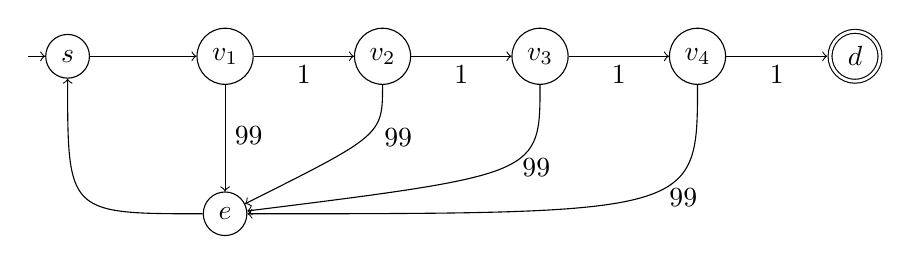
\begin{tikzpicture}[main/.style = {draw, circle},double_border/.style={draw, double, double distance=1pt,outer sep=1pt}] 
        \node[main] (1) at (0,0) {$s$};
        \node[main] (2) at (2, 0) {$v_1$};
        \node[main] (3) at (4, 0){$v_2$};
        \node[main] (4) at (6, 0) {$v_3$};
        \node[main] (5) at (8, 0) {$v_4$};
        \node[main,double_border] (6) at (10, 0) {$d$};
        \node[main] (7) at (2, -2) {$e$};
        \draw[->] (1) -- (2);
        \draw[->] (2) -- node[below] {$1$} (3);
        \draw[->] (3) -- node[below] {$1$} (4);
        \draw[->] (4) -- node[below] {$1$} (5);
        \draw[->] (5) -- node[below] {$1$} (6);
        \draw[->] (5) .. controls +(down:2) .. node[align=right,right] {\ \ $99$} (7);
        \draw[->] (4) .. controls +(down:1.5) .. node[right] {\ $99$} (7);
        \draw[->] (3) .. controls +(down:1) .. node[right] {\ $99$} (7);
        \draw[->] (2) .. controls +(down:1) .. node[right] {$99$} (7);
        \draw[->] (7) .. controls +(left:2) ..  (1);
        \draw[->] (-0.5,0) -- (1);
    \end{tikzpicture} 
    \caption{Zustandsgraf einer fiktiven Anwendung mit Validierung, einem transaktionalen Arbeitsablauf und einem hohen Verzweigungsgrad. $s$ ist der Startzustand, $d$ ist der Zielzustand, $e$ ist ein Fehlerzustand. Die Zahlen an den Kanten stehen für die Anzahl der möglichen Benutzerinteraktionen, die den Zustandsübergang auslösen. Die Wahrscheinlichkeit, dass ein Monkey-Tester den Zielzustand und nicht erneut den Startzustand erreicht, ist lediglich Eins in hundert Millionen.}
    \label{fig:sad_monkey}
\end{figure}

Eine Art von Anwendung, die diese Anforderungen erfüllen kann, sind Webshops:
Webshops enthalten eine Vielzahl von Interaktionselementen, wie Produktlisten, Warenkörbe und Kassenprozesse.
Sie enthalten transaktionale Arbeitsabläufe, wie das Hinzufügen von Produkten zum Warenkorb gefolgt von einer Bestellung.
Sie enthalten Validierungslogik, zum Beispiel bei dem Ausfüllen von Adressfeldern.
Sie haben einen hohen Verzweigungsgrad, da es viele verschiedene Produkte gibt, die zu verschiedenen Anwendungszuständen führen.
Außerdem sind sie praxisrelevant: Der Marktanteil von E-Commerce ist groß und wächst weiter.
\footnote{
Der Anteil von E-Commerce am Einzelhandelsumsatz in den USA betrug im Quartal 1, 2023 15,6\%. U.S. Bureau of the Census über FRED, Federal Reserve Bank of St. Louis. \url{https://fred.stlouisfed.org/series/ECOMPCTSA}}
Und erfreulicherweise sind ihre GUIs in der Regel Webseiten, sodass die textuelle Repräsentation ihrer GUI, das HTML-Dokument, direkt verfügbar ist.

Um eine geeignete Anwendung zu finden, habe ich eine Reihe von Open-Source-Projekten durchsucht, die als Webshop-Software oder Template für solche vermarktet werden.
Eine Auswahl dieser Projekte ist in Abbildung \ref{tab:webshop_projects} aufgeführt.

\begin{figure}[h]
    \begin{minipage}[c]{\textwidth}
        \centering
        {
            \scriptsize
            \begin{tabular}{ | l | l | l | l | l |}
                \hline
                \textbf{Projekt} & \textbf{Letzter Commit} & \textbf{Lizens} & \textbf{Technologie} & \textbf{Vermerk} \\ \hline
                Online Shopping Cart\footnote{\url{https://github.com/shashirajraja/shopping-cart}} & Mai 23 & Apache 2 & Java, Servlets, JSP, SQL & Demonstrationszweck \\ \hline
                LifestyleStore\footnote{\url{https://github.com/sajalagrawal/LifestyleStore}} & August 20 & - & PHP, SQL & Lernzweck \\ \hline
                Your Online Shop\footnote{\url{https://github.com/petazeta/youronlineshop}} & Dezember 22 & custom & Node.js, MongoDB & - \\ \hline
                Ecommerce-Website\footnote{\url{https://github.com/winston-dsouza/ecommerce-website}} & Februar 20 & MIT & PHP, SQL & keine transaktionalen Workflows \\ \hline
                Book-Hub\footnote{\url{https://github.com/amberkakkar01/Book-Hub}} & August 21 & - & HTML & statisches HTML \\ \hline
                online-shopping-site\footnote{\url{https://github.com/dinushchathurya/online-shopping-site}} & Mai 19 & GPLv3 & JavaScript & ohne Server \\ \hline
                Online-Fashion-Store\footnote{\url{https://github.com/RazaRizvii/Online-Fashion-Store}} & Dezember 22 & - & JavaScript & ohne Server \\ \hline
                online-shopping-website\footnote{\url{https://github.com/nsk1512/online-shopping-website}} & Dezember 19 & - & Node.js, MongoDB & - \\ \hline
                Ketra-Mart\footnote{\url{https://github.com/Prajwal100/ketra-mart-free}} & Juni 23 & MIT & ? & Quellcode nur gegen Zahlung \\ \hline
                Shuup\footnote{\url{https://github.com/shuup/shuup}} & August 21 & OSL & Python, SQL & Kommerziell, Multi-Vendor \\ \hline
                EverShop\footnote{\url{https://github.com/evershopcommerce/evershop}} & September 23 & GPLv3 & Node.js, SQL & - \\ \hline
                Hayroo\footnote{\url{https://github.com/hasan-py/MERN_Stack_Project_Ecommerce_Hayroo}} & May 23 & - & Node.js, MongoDB & - \\ \hline
            \end{tabular}
        }
    \end{minipage}
    \caption{Open-source Webshop Projekte, die für die Verwendung in dieser Arbeit gesichtet wurden.}
    \label{tab:webshop_projects}
\end{figure}

Die meisten dieser Projekte sind nicht für die Verwendung in dieser Arbeit geeignet, da sie entweder nicht transaktional sind oder keine passende Lizenz haben.
\textit{EverShop} und \textit{Shuup} erfüllen zwar alle Anforderungen, sind aber so komplex und umfangreich, dass ein maßgeblicher Teil der Arbeit darin bestehen würde, die Anwendung zu verstehen und zu modifizieren, um sie für die Evaluation des Ansatzes zu verwenden.
\textit{online-shopping-website} hingegen ist streng genommen nicht für den praktischen Einsatz gedacht, erfüllt aber fast alle Anforderungen und ist klein und simpel.
Nur eine Möglichkeit zur Kaufabwicklung mit einer validierten Eingabemaske fehlt, welche aber mit vertretbarem Aufwand hinzugefügt werden kann.
Deshalb wurde entschieden, eine eigene Anwendung auf Basis von \textit{online-shopping-website} zu entwickeln, die alle Anforderungen erfüllt und gleichzeitig einfach genug ist, um sie in der verfügbaren Zeit zu evaluieren.

\section{Forschungsfragen}

\begin{enumerate}
    \item Can LLMs understand HTML?
    \item Feasibility of the approach
    \item Do you need the whole document? / Advantage of “stripped tree”
    \item Flakiness > Repeats necessary / how many?
    \item Optional: Possibility and Accuracy of validation
    \item Optional: Impact of prompt engineering?
\end{enumerate}

\section{Getestete Anwendung}

Um die Methode des automatisierten Testens von Webanwendungen mit LLMs zu evaluieren, habe ich eine eigene Anwendung entwickelt, die als Testanwendung dient.
Diese Testanwendung ist ein Webshop, in dem Benutzer mit verschiedenen Elementen interagieren können, wie Produktlisten für verschiedene Produktkategorien, einem Warenkorb und dem Kassenprozess.

Als Grundlage für die Testanwendung dient das Open-Source Projekt \textit{online-shopping-website} \footnote{\url{https://github.com/nsk1512/online-shopping-website}}.
\textit{online-shopping-website} enthält bereits eine Startseite, Produktlisten und einen Warenkorb.
Die Anwendung ist in JavaScript geschrieben und benötigt keine externen Abhängigkeiten, Server oder Datenbanken.
Für diese Arbeit habe ich die Anwendung unter Verwendung der Bibliothek \textit{react}\footnote{\url{https://react.dev/}} neu implementiert und um eine Kassenfunktionalität, Validierungslogik und eine Bestellbestätigungsseite erweitert.
Mit diesen Erweiterungen erfüllt die Anwendung alle Anforderungen, die am Anfang dieses Kapitels aufgeführt sind.

Die Webseite ist jetzt wie folgt aufgebaut:
Es gibt vier verschiedene Seiten, die der Benutzer besuchen kann: Die Startseite, die Produktlisten für verschiedene Produktkategorien, die Kasse und die Bestellbestätigungsseite.
Diese sind in Abbildung \ref{fig:online-shopping-website} dargestellt.
Jede Seite enthält eine Titelleiste mit einem aufklappbaren Menü, das den Benutzer zu den anderen Seiten führt und eine aufklappbare Warenkorbansicht.
Die Produktlisten und die Startseite enthalten Bilder, Namen und Preise der Produkte und eine Schaltfläche, um das Produkt zum Warenkorb hinzuzufügen.
Die Startseite enthält ausgewählte Produkte aus verschiedenen Kategorien und eine Schaltfläche um zu einer hervorgehobenen Produktkategorie zu gelangen.
In dem aufklappbaren Warenkorb lassen sich die Produkte entfernen und die Anzahl der Produkte ändern und es gibt eine Schaltfläche, um zur Kasse zu gelangen.
In der Kasse gibt es eine Bestellübersicht und dort gibt der Benutzer seine Adresse und Zahlungsdaten ein und bestätigt die Bestellung.
Daraufhin werden die Benutzereingaben auf Vollständigkeit und korrekte Form validiert.
Falls sie korrekt sind, gelangt der Nutzer zur Bestellbestätigungsseite, sonst wird er aufgefordert, die Eingaben entsprechend zu korrigieren.

\begin{figure}
    \centering
    \begin{subfigure}[b]{0.32\textwidth}
        \centering
        \includegraphics[width=\textwidth]{pictures/Start.png}
        \caption{Startseite}
        \label{fig:online-shopping-website-start}
    \end{subfigure}
    \hfill
    \begin{subfigure}[b]{0.32\textwidth}
        \centering
        \includegraphics[width=\textwidth]{pictures/Leiste.png}
        \caption{auf\-ge\-klappte Titelleiste}
        \label{fig:online-shopping-website-menu}
    \end{subfigure}
    \hfill
    \begin{subfigure}[b]{0.32\textwidth}
        \centering
        \includegraphics[width=\textwidth]{pictures/Cart.png}
        \caption{Warenkorb}
        \label{fig:online-shopping-website-cart}
    \end{subfigure}
    
    % New row
    \begin{subfigure}[b]{0.9\textwidth}
        \centering
        \includegraphics[width=\textwidth]{pictures/Products_Half.png}
        \caption{Produktliste}
        \label{fig:online-shopping-website-product-list}
    \end{subfigure}
    \begin{subfigure}[b]{0.9\textwidth}
        \centering
        \includegraphics[width=\textwidth]{pictures/Checkout.png}
        \caption{Kasse}
        \label{fig:online-shopping-website-checkout}
    \end{subfigure}

    \caption{Screenshots der Testanwendung}
    \label{fig:online-shopping-website}
\end{figure}

\section{Extraktion von Interaktionsmöglichkeiten}

Für das Testen mittels LLM ist es notwendig, die möglichen Benutzerinteraktionen aus der HTML-Repräsentation der Anwendung zu extrahieren.
Ein Monkey-Tester könnte die Interaktionselemente zwar auch durch rein zufällige Maus und Tastaturaktionen finden, dann wären die Testergebnisse nicht mehr vergleichbar mit denen des LLMs.

Leider genügt es nicht, Interaktionselemente durch ihre HTML-Tags und -Attribute zu identifizieren, denn in der Praxis ist es schwierig, die Interaktionselemente zu identifizieren, die nicht verdeckt sind.
Außerdem ist es mittels JavaScript möglich und gängig, auch HTML-Elemente interagierbar zu machen, die nicht dazu gedacht sind.
Beispielsweise sind einige Knöpfe in der Testanwendung keine HTML-Buttons, sondern div-Elemente, die durch JavaScript-Event-Listener interagierbar sind.
Rein auf Basis des HTML-Dokuments ist es nicht möglich, zu erkennen, dass diese Elemente interagierbar sind.

Ich habe keine Möglichkeit gefunden, automatisch festzustellen, welche Elemente einer Webseite interagierbar sind.
Deshalb habe ich die Verantwortlichkeit für die Identifikation dieser Elemente auf den Entwickler der zu testenden Anwendung gelegt.
Für das Testframework, das ich entwickelt habe, ist es notwendig, dass benutzbare HTML-Elemente durch ein spezielles Attribut gekennzeichnet sind.

Um herauszufinden, welche dieser gekennzeichneten Elemente nicht verdeckt sind, habe ich ein Skript entwickelt, das mithilfe der Bibliothek \textit{Selenium}\footnote{\url{https://www.selenium.dev/}} direkt im Browser ausgeführt wird.
Es benutzt die DOM-API des Browsers, um abzufragen, welches Element an der Stelle eines gekennzeichneten Elements zu oberst liegt.
Das gekennzeichnete Element kann nicht verdeckt sein, wenn das oberste Element Nachfahre des gekennzeichneten Elements oder das Element selbst ist.
Für die Testanwendung reicht dieses Kriterium zwar aus, generell lassen sich aber Fälle konstruieren, in denen dieses Kriterium nicht ausreicht, oder nicht zutrifft:
Beispielsweise durch absolute Positionierung oder z-index kann es sein, dass ein Element, das nicht vollständig verdeckt ist, nicht als solches erkannt wird.
Oder wenn das gekennzeichnete Element vollständig von Kindelementen verdeckt ist, die selbst interagierbar sind, ist das gekennzeichnete Element nicht interagierbar.

\section{Prompt-Engineering}

Die Qualität der generierten Ausgabe eines LLM hängt stark von der Qualität der Eingabe ab, die dem LLM gegeben wird. \cite{chain-of-thought}
Prompt-Engineering ist die Kunst, eine Eingabe zu formulieren, die das gewünschte Verhalten des LLM hervorruft.
In dieser Arbeit habe ich mich auf die Entwicklung von Prompts konzentriert, die die Anwendung navigieren und testen.
Im Speziellen sind Eingaben, mit denen das LLM zu Anwendungszuständen navigiert, die von klassischen Monkey-Testern schwer zu erreichen sind, von Interesse.

Dazu vergleiche ich die Qualität der generierten Benutzerinteraktionen, wenn das LLM mit verschiedenen Eingabe aufgerufen wird.
Die Qualität der generierten Benutzerinteraktionen wird anhand der Branchenabdeckung gemessen, mehr dazu in Abschnitt \ref{sec:vaildation}.

\begin{enumerate}
    \item Basis-Eingabe: Die Basis-Eingabe ist ein einfacher Satz, der das LLM auffordert, eine Benutzerinteraktion zu generieren die eine gegeben Webanwendung testen soll.
    \\
    Beispieleingabe:
    \\
    \textit{Du bist Tester für Webanwendungen und sollst eine gegebene Anwendung möglichst ausführlich Testen.
    Hier ist die HTML-Repräsentation der Anwendung: ...
    Antworte mit einer der folgenden Benutzerinteraktionen: Klick auf \dq weiter\dq, Klick auf \dq zurück\dq.}
    \item Verkettung: Zusätzlich zu der Basis-Eingabe wird jeweils die letzte Ausgabe des LLMs an die Eingabe angefügt.
    \\
    Beispieleingabe:
    \\
    \textit{System: Du bist Tester für Webanwendungen und sollst eine gegebene Anwendung möglichst ausführlich Testen.
    Hier ist die HTML-Repräsentation der Anwendung: ...
    Antworte mit einer der folgenden Benutzerinteraktionen: Klick auf \dq weiter\dq, Klick auf \dq zurück\dq.
    \\
    LLM: Klick auf \dq weiter\dq
    \\
    System: Hier ist die neue HTML-Repräsentation der Anwendung: ... Bitte fahre mit dem Testen fort. Antworte mit einer der folgenden Benutzerinteraktionen: Klick auf \dq weiter\dq, Klick auf \dq zurück\dq.
    }
    \item Beschreibung: Zusätzlich zur Verkettung wird das LLM aufgefordert eine Beschreibung des Anwendungszustands zu generieren. Diese wird dann mit in folgenden Eingaben verkettet.
    \\
    Beispieleingabe:
    \\
    \textit{System: Du bist Tester für Webanwendungen und sollst eine gegebene Anwendung möglichst ausführlich Testen.
    Hier ist die HTML-Repräsentation der Anwendung: ... 
    Gib eine kurze Beschreibung des Anwendungszustands an, dann antworte mit einer der folgenden Benutzerinteraktionen: Klick auf \dq weiter\dq, Klick auf \dq zurück\dq.
    \\
    LLM: Es wird ein Dialog mit dem Warnhinweis angezeigt, dass die Löschung des Benutzerkontos endgültig ist. Klick auf \dq weiter\dq
    \\
    System: Hier ist die neue HTML-Repräsentation ...
    }
    \item Begründung: Das Model wird dazu aufgefordert eine Begründung für die Entscheidung zur Nutzerinteraktion zu liefern.
    \\
    Beispieleingabe:
    \\
    \textit{System: Du bist Tester für Webanwendungen und sollst eine gegebene Anwendung möglichst ausführlich Testen.
    Hier ist die HTML-Repräsentation der Anwendung: ... 
    Gib eine kurze Beschreibung des Anwendungszustands an, dann antworte mit einer einem Plan was als nächstes getestet werden soll und einer der folgenden Benutzerinteraktionen, die dafür gewählt werden muss: Klick auf \dq weiter\dq, Klick auf \dq zurück\dq. 
    \\
    LLM: Es wird ein Dialog mit dem Warnhinweis angezeigt, dass die Löschung des Benutzerkontos endgültig ist.
    Teste das Löschen des Benutzerkontos.
    Klick auf \dq weiter\dq
    \\
    System: Hier ist die neue HTML-Repräsentation ...
    }
    \item Selbst-Formulierte Ziele: Das LLM wird dazu aufgefordert Ziele zu formulieren, die es in der Anwendung erreichen soll. Diese Ziele sollen mehrere Benutzerinteraktionen umfassen.
    \item 
    \item Chain of Thought Eingaben: Das erwartete Format für die Ausgabe des LLM enthält einen kompletten erklärenden Gedankengang. Dazu werden Beispiele im Prompt geliefert \cite{chain-of-thought}.
\end{enumerate}

\section{Resultate}
\label{sec:vaildation}

\begin{figure}
    \centering
    \begin{tikzpicture}
        \begin{axis}[
            ymajorgrids=true,
            xmin=0, xmax=100,
            grid style=dashed,
            width=0.9\textwidth,
            ylabel={Branchenabdeckung [\%]},
            xlabel={Anzahl der generierten Benutzerinteraktionen [1]},
            no markers,
            legend pos=south east,
            %xtick=data,
            ]
            \addplot[color=green] table [x=x,y=average,col sep=comma] {experimental_data/monkey/results.csv};
            \label{Monkey-Testing, n=10}
            \addplot+[forget plot,name path=monkey_top,color=green!70] table [x=x,y=above,col sep=comma] {experimental_data/monkey/results.csv};
            \addplot+[forget plot,name path=monkey_bottom,color=green!70] table [x=x,y=below,col sep=comma] {experimental_data/monkey/results.csv};
            \addplot+[forget plot,green!50,fill opacity=0.5] fill between[of=monkey_top and monkey_bottom];
            \addlegendentry{Monkey-Testing, n=10}

            \addplot[color=blue] table [x=x,y=average,col sep=comma] {experimental_data/gpt4-base/results.csv};
            \addlegendentry{GPT-4 Basiseingabe, n=4}
            \label{Basis-Eingabe, n=4}
        \end{axis}
    \end{tikzpicture}
    
\end{figure}

\iffalse
\chapter{Execution}

\section{Riscs}

\section{Schedule}

\ganttset{%
    calendar week text={%
        \currentweek
    }%
}
\begin{ganttchart}[hgrid,
time slot format=isodate,
    x unit=2pt,]{2023-06-12}{2023-12-11}
    \gantttitlecalendar{year, month, week}\\
    %\gantttitle{2023-06-12}{2024-01-1} \\
    %\gantttitlelist{1,...,12}{1} \\
    \ganttbar{Lit. Research}{2023-06-12}{2023-06-26} \\%2
    \ganttgroup{Implementation}{2023-06-26}{2023-08-21} \\
    \ganttbar{AUT}{2023-06-26}{2023-07-24} \\%4
    \ganttbar{Implementation}{2023-07-24}{2023-08-21} \\%4
    \ganttgroup{Validation}{2023-08-21}{2023-10-02} \\
    \ganttbar{Design Tests}{2023-08-21}{2023-09-04} \\%2
    \ganttbar{GPT3}{2023-09-04}{2023-09-11} \\%1
    \ganttbar{GPT4}{2023-09-11}{2023-09-18} \\%1
    \ganttbar{Monkey Testing}{2023-09-18}{2023-10-02} \\%2
    %\ganttbar{open source GPT}{2023-10-09}{2023-10-23} \\
    %\ganttbar{Monkey Testing}{2023-10-09}{2023-10-23} \\
    \ganttgroup{Documentation}{2023-10-02}{2023-11-27} \\%4
    \ganttbar{Writing}{2023-10-02}{2023-11-13} \\%6
    \ganttbar{Finalize}{2023-11-13}{2023-11-27} \\%2
    \ganttbar{Buffer}{2023-11-27}{2023-12-11}%2
    %\ganttbar{Final Task}{8}{12}
    %\ganttlink{elem2}{elem3}
    %\ganttlink{elem3}{elem4}
\end{ganttchart}
\fi

%% ---------------------
%% | / Example content |
%% ---------------------
%% LaTeX2e class for student theses
%% sections/conclusion.tex
%% 
%% Karlsruhe Institute of Technology
%% Institute for Program Structures and Data Organization
%% Chair for Software Design and Quality (SDQ)
%%
%% Dr.-Ing. Erik Burger
%% burger@kit.edu
%%
%% Version 1.3.6, 2022-09-28



\newcommand{\minipicture}[3]{
    \begin{tikzpicture}
        \begin{axis}[
            ymajorgrids=true,
            xmin=0, xmax=#3,
            grid style=dashed,
            ylabel={Abdeckung [\%]},
            xlabel={Interaktionen [1]},
            width=#2,
            no markers,
            ]
            
            \addplot[color=green] table [x=x,y=average,col sep=comma] {experimental_data/monkey/results.csv};
            \addplot+[forget plot,name path=monkey_top,color=green!70] table [x=x,y=above,col sep=comma] {experimental_data/monkey/results.csv};
            \addplot+[forget plot,name path=monkey_bottom,color=green!70] table [x=x,y=below,col sep=comma] {experimental_data/monkey/results.csv};
            \addplot+[forget plot,green!50,fill opacity=0.5] fill between[of=monkey_top and monkey_bottom];

            \addplot[color=black] table [x=x,y=average,col sep=comma] {experimental_data/#1/results.csv};
            \addplot+[forget plot,name path=#1_top,color=black!70] table [x=x,y=above,col sep=comma] {experimental_data/#1/results.csv};
            \addplot+[forget plot,name path=#1_bottom,color=black!70] table [x=x,y=below,col sep=comma] {experimental_data/#1/results.csv};
            \addplot+[forget plot,black!50,fill opacity=0.5] fill between[of=#1_top and #1_bottom];
        \end{axis}
    \end{tikzpicture}
}

\newcommand{\miniplot}[4]{
    \begin{subfigure}[b]{0.47\textwidth}
        \minipicture{#1}{\textwidth}{#4}
        \caption{#2}
        \label{fig:#3}
    \end{subfigure}
}

\chapter{Ergebnisse}
\label{ch:Results}

\begin{figure}
    % 25 interactions
    \centering
    \begin{tabular}{|l|c|c|c|c|c|c|}
        \hline
        Modell & Eingabe & n & \multicolumn{4}{c|}{Branchenabdeckung [\%]}  \\
         &  &  & Mittel & Min & Max & $\sigma$ \\
        \hline
        Monkey & - & 10 & 71,2 & 60,2 & 78,6 & 4,8 \\
        GPT-3.5 & Verkettung & 4 & 65,8 & 56,1 & 70,4 & 5,7 \\
        GPT-3.5 & Beschreibung & 4 & 67,9 & 58,2 & 75,5 & 6,3 \\
        GPT-3.5 & Erklärung & 4 & 60,2 & 54,1 & 67,3 & 5,1 \\
        GPT-3.5 & Ziele & 5 & 61,8 & 52 & 68,4 & 6,3 \\
        GPT-3.5 & Chain of Thought & 4 & 68,6 & 57,1 & 74,5 & 6,9 \\
        GPT-4 & Verkettung & 2 & 74,0 & 73,5 & 74,5 & 0,5 \\
        GPT-4 & Beschreibung & 3 & 66,0 & 62,2 & 73,5 & 5,3 \\
        GPT-4 & Erklärung & 5 & 77,6 & 74,5 & 79,6 & 2,1 \\
        GPT-4 & Ziele & 4 & 79,1 & 75,5 & 83,7 & 3,3 \\
        GPT-4 & Chain of Thought & 4 & 81,4 & 78,6 & 87,8 & 3,8 \\
        \hline
    \end{tabular}
    \caption{Zusammenfassung der Ergebnisse der Tests mit den Sprachmodellen und Monkey-Testing nach 25 Interaktionen.}
    \label{tab:results}
\end{figure}



\section{Erste Tests mit GPT-3.5 und der ursprünglichen Eingabe}

Nach der Implementierung des Systems wurden zuerst Tests mit GPT-3.5 durchgeführt, um die Funktionalität des Systems zu überprüfen; Übersicht der Ergebnisse siehe Abbildung \ref{tab:results}.
Dabei wurde eine Eingabe verwendet, die der von \Citeauthor{GPT3Testing} nachempfunden ist:
Darin wird das LLM aufgefordert, zuerst eine Benutzerinteraktion zu generieren und dann eine Begründung zu liefern, warum diese Benutzerinteraktion generiert wurde.
Die gleiche Eingabe lässt sich nicht verwenden, da in meiner Implementierung mehr Arten von Benutzerinteraktionen unterstützt werden und die Ausgabe anders aufgebaut sein muss.
Ergebnisse von Tests mit dieser Eingabe sind in Abbildung \ref{fig:gpt3_5_explain_after} zu sehen.
Mit dieser Eingabe war die Branchenabdeckung nach 25 Interaktionen mit durchschnittlich $55{,}7\%$ deutlich niedriger als die von Monkey-Testing mit durchschnittlich $71{,}2\%$.

Ein Problem, das bei diesen Tests auftrat, war, dass das LLM oft identische Benutzerinteraktionen mehrfach in Folge generierte.
Beispielsweise wurde mehrmals hintereinander mit jeweils identischer Begründung auf die Schaltfläche \enquote{Submit} geklickt.
Angesichts dessen, dass GPT-3.5 in anderen Anwendungsgebieten gute Ergebnisse erzielt, war das Ergebnis enttäuschend und ich entschied, Eingaben zu suchen, die zu besseren Ergebnissen führen könnten.
Die Resultate dieser Suche sind die in Abschnitt \ref{sec:prompt-engineering} beschriebenen Eingaben.

\begin{figure}[h]
    \centering
    \minipicture{gpt3-5-explain-after}{0.47\textwidth}{25}
    \caption{Ergebnisse der Tests mit GPT-3.5 und einer Eingabe, die verlangt erst eine Benutzerinteraktion und dann eine Begründung zu generieren. Die schwarze Linie zeigt die durchschnittliche Branchenabdeckung, die grüne Linie zeigt die durchschnittliche Branchenabdeckung von Monkey-Testing. Der schattierte Bereich um die Linien zeigt die Standardabweichung.}
    \label{fig:gpt3_5_explain_after}
\end{figure}

\section{Suche nach besseren Eingaben für GPT-3.5}
\label{sec:prompt-engineering:2}


\begin{figure}
    \centering
    \begin{tikzpicture}
        \begin{axis}[
            ymajorgrids=true,
            xmin=0, xmax=25,
            grid style=dashed,
            width=0.9\textwidth,
            ylabel={durchschnittliche Branchenabdeckung [\%]},
            xlabel={Anzahl der generierten Benutzerinteraktionen [1]},
            no markers,
            legend pos=south east,
            %xtick=data,
            ]
            \addplot[color=green] table [x=x,y=average,col sep=comma] {experimental_data/monkey/results.csv};
            \addlegendentry{Monkey-Testing, n=10}

            \addplot[color=black] table [x=x,y=average,col sep=comma] {experimental_data/gpt3-5-base/results.csv};
            \addlegendentry{GPT-3.5 Basiseingabe, n=1}

            \addplot[color=red] table [x=x,y=average,col sep=comma] {experimental_data/gpt3-5-chained/results.csv};
            \addlegendentry{GPT-3.5 Verkettung, n=4}

            \addplot[color=blue] table [x=x,y=average,col sep=comma] {experimental_data/gpt3-5-description/results.csv};
            \addlegendentry{GPT-3.5 Beschreibung, n=4}

            \addplot[color=cyan] table [x=x,y=average,col sep=comma] {experimental_data/gpt3-5-explain/results.csv};
            \addlegendentry{GPT-3.5 Erklärung, n=4}

            \addplot[color=orange] table [x=x,y=average,col sep=comma] {experimental_data/gpt3-5-goals/results.csv};
            \addlegendentry{GPT-3.5 Ziele, n=5}

            \addplot[color=magenta] table [x=x,y=average,col sep=comma] {experimental_data/gpt3-5-chain-of-thought/results.csv};
            \addlegendentry{GPT-3.5 Chain of Thought, n=4}
        \end{axis}
    \end{tikzpicture}
    \caption{Vergleich der durchschnittlich gemessenen Branchenabdeckung von GPT-3.5 mit allen Eingaben und Monkey-Testing.}
    \label{fig:gpt3_5_all}
\end{figure}

\begin{figure}
    \centering
    \miniplot{gpt3-5-base}{GPT-3.5 Basiseingabe, n=1}{gpt3_5_base}{25}\hfill
    \miniplot{gpt3-5-chained}{GPT-3.5 Verkettung, n=4}{gpt3_5_chained}{25}
    \miniplot{gpt3-5-description}{GPT-3.5 Beschreibung, n=4}{gpt3_5_describe}{25}\hfill
    \miniplot{gpt3-5-explain}{GPT-3.5 Erklärung, n=4}{gpt3_5_explain}{25}
    \miniplot{gpt3-5-goals}{GPT-3.5 Ziele, n=5}{gpt3_5_goals}{25}\hfill
    \miniplot{gpt3-5-chain-of-thought}{GPT-3.5 Chain of Thought, n=4}{gpt3_5_chain_of_thought}{25}
    \caption{Vergleich der durchschnittlich gemessenen Branchenabdeckung von GPT-3.5 (schwarz) und Monkey-Testing (grün). Der schattierte Bereich um die Linien zeigt die Standardabweichung.}
\end{figure}

Die erste Eingabe, die ich ausprobierte, war die Basiseingabe, bei der dem LLM nicht die Ein- und Ausgaben vorheriger Interaktionen gegeben werden.
Das führt zu noch schlechteren Ergebnissen, wie in Abbildungen \ref{fig:gpt3_5_all} und \ref{fig:gpt3_5_base} zu sehen ist.
Der LLM-Tester führt bei gleichem Zustand fast immer die gleiche Aktion aus, was dazu führt, dass er in Schleifen von ein bis zwei Interaktionen stecken bleibt und keine neuen Aktionen ausführt.

Die nächste Eingabe, die ich ausprobierte, war die Verkettung, bei der dem LLM die Ein- und Ausgaben vorheriger Interaktionen mit in die Eingabe gegeben werden.
Die Ergebnisse dieser Eingabe sind in Abbildung \ref{fig:gpt3_5_chained} zu sehen.
Mit dieser Eingabe war die Branchenabdeckung nach 25 Interaktionen schon $65{,}8\%$, auch wenn der Unterschied zur ursprünglichen Eingabe nur das Fehlen der Forderung nach einer Begründung ist.

Fordert man vor der Benutzerinteraktion eine Beschreibung der Webseite, steigt die Branchenabdeckung auf $67{,}9\%$ und es scheint, als ob nicht mehr viel fehlen würde, um die Branchenabdeckung von Monkey-Testing zu erreichen.
Die nächste Ergänzung der Eingabe, das Fordern einer Erklärung, was mit der Benutzerinteraktion erreicht werden soll, führte aber wieder zu einer deutlichen Verschlechterung der Ergebnisse, wie in Abbildung \ref{fig:gpt3_5_explain} zu sehen ist.

Ein Hauptproblem mit dieser Eingabe scheint zu sein, dass das Sprachmodell die Webseite nicht versteht und deshalb nicht in der Lage ist, sinnvolle Handlungsabläufe zu generieren:
Beispielsweise wurde immer wieder die Erklärung \enquote{\foreignlanguage{english}{Proceed with the checkout process by submitting the payment information.}} (Deutsch: \enquote{Fahre mit dem Bezahlvorgang fort, indem die Zahlungsinformationen abgeschickt werden.}) generiert, obwohl die Zahlungsinformationen nicht gesondert vom Rest des Bestellvorgangs abgeschickt werden können.
Ferner beachtete das Sprachmodell auch die daraufhin auf der Webseite erscheinende Fehlermeldung nicht und versuchte immer wieder das halb ausgefüllte Formular abzuschicken.

In einem anderen Test versucht das Sprachmodell immer wieder den \enquote{Pfeil nach oben}-Knopf im Warenkorb (Abbildung \ref{fig:online-shopping-website-cart}) zu drücken, mit dem die Menge eines Artikels erhöht werden kann, um eine nähere Beschreibung dieses Artikels zu erhalten.
Das kommt vermutlich daher, dass die textuelle Repräsentation dieses Knopfes den Schriftzug \enquote{fa-cart-plus} enthält, was das Sprachmodell scheinbar als Indiz dafür interpretiert, dass es sich um einen Knopf für eine Detailansicht handelt.
(Danach folgt \enquote{fa-cart-minus}, somit ist diese Interpretation unwahrscheinlich.)

Ein anderes Problem ist, dass in einigen Fällen die erzeugte Handlungsabsicht nicht in einer Benutzerinteraktion ausführbar ist, beispielsweise wurde die Handlungsabsicht \enquote{\foreignlanguage{english}{To test the checkout process, simulate clicking on the 'Checkout' button in the cart overlay.}} (Deutsch: \enquote{Um den Bezahlvorgang zu testen, simuliere das Klicken auf den 'Checkout'-Knopf im Warenkorb-Overlay.}) generiert, obwohl das Warenkorb-Overlay nicht geöffnet war und somit der Knopf nicht existierte.
Die Eingabe verlangt aber, dass die Handlungsabsicht mit der Benutzerinteraktion ausgeführt werden soll, daher werden solche Handlungsabsichten ignoriert oder führen zu fehlerhaften Benutzerinteraktionen.

Um diese Probleme zu lösen, hatte ich die Idee, dass das Sprachmodell sich selbst Ziele setzen sollte, die es mit den nächsten Benutzerinteraktionen erreichen will.
Falls ein Ziel nicht mehr erreichbar scheint, sollte das Sprachmodell neue Ziele formulieren.
Gleichzeitig bekommt das Sprachmodell eine Auflistung der Ziele, die es sich zuvor gesetzt hat, und wie viele Benutzerinteraktionen es für jedes Ziel schon generiert hat.
Die Ergebnisse dieser Eingabe sind in Abbildung \ref{fig:gpt3_5_goals} zu sehen; diese Eingabe führte zu keiner relevanten Verbesserung der Ergebnisse.
Ein Hauptproblem war, dass das LLM fast bei jeder Benutzerinteraktion ein neues Ziel setzte, was dazu führte, dass es nie genug Benutzerinteraktionen für ein Ziel generierte, um es zu erreichen.

Die letzte Eingabe, die ich ausprobierte, war die \enquote{Chain of Thought}-Eingabe, bei der das Sprachmodell neben den, bei den anderen Eingaben erzeugten Gedankengängen, auch Beispiele für gute Gedankengänge und Benutzerinteraktion bekommt.
Diese Beispiele sind für andere Webseiten als die Testwebseite, um dem Sprachmodell keinen unfairen Vorteil gegenüber Monkey-Testing zu verschaffen.
Tatsächlich führte diese Eingabe zu einer Verbesserung der Ergebnisse, durchschnittlich erreichte das LLM damit eine Branchenabdeckung von $68{,}6$, wie in Abbildung \ref{fig:gpt3_5_chain_of_thought} zu sehen ist.
Der Unterschied der Branchenabdeckung zu Monkey-Testing ist relativ gering, und in einigen Fällen ist die Branchenabdeckung von GPT-3.5 höher als die von Monkey-Testing.

Insgesamt war das Ergebnis dieser Tests, dass die von mir definierten Eingaben zu einer Verbesserung der Ergebnisse führten, aber zumindest bei GPT-3.5 nicht ausreichten, um die Branchenabdeckung von Monkey-Testing zu übertreffen.
In einigen Tests hat das Sprachmodell den Bestellprozess, der ein Beispiel für eine für Monkey-Tester schwierige transaktionale Interaktion wie in Abbildung \ref{fig:sad_monkey} ist, teilweise durchgespielt.
Aber es wurde nie eine Bestellung abgeschlossen, während der Monkey-Tester ähnliche oder höhere Branchenabdeckung erreichte.
Es wurden auch keine Texteingaben generiert, die zu Validierungsfehlern führten, obwohl das Sprachmodell in der Eingabe dazu aufgefordert wurde, nach Randfällen zu suchen.


\section{Tests mit GPT-4}


\begin{figure}
    \centering
    \begin{tikzpicture}
        \begin{axis}[
            ymajorgrids=true,
            xmin=0, xmax=100,
            grid style=dashed,
            width=0.9\textwidth,
            ylabel={durchschnittliche Branchenabdeckung [\%]},
            xlabel={Anzahl der generierten Benutzerinteraktionen [1]},
            no markers,
            legend pos=south east,
            %xtick=data,
            ]
            \addplot[color=green] table [x=x,y=average,col sep=comma] {experimental_data/monkey/results.csv};
            \addlegendentry{Monkey-Testing, n=10}

            \addplot[color=black] table [x=x,y=average,col sep=comma] {experimental_data/gpt4-base/results.csv};
            \addlegendentry{GPT-4 Basiseingabe, n=1}

            \addplot[color=red] table [x=x,y=average,col sep=comma] {experimental_data/gpt4-chained/results.csv};
            \addlegendentry{GPT-4 Verkettung, n=2}

            \addplot[color=blue] table [x=x,y=average,col sep=comma] {experimental_data/gpt4-describe/results.csv};
            \addlegendentry{GPT-4 Beschreibung, n=3}

            \addplot[color=cyan] table [x=x,y=average,col sep=comma] {experimental_data/gpt4-explain/results.csv};
            \addlegendentry{GPT-4 Erklärung, n=5}

            \addplot[color=magenta] table [x=x,y=average,col sep=comma] {experimental_data/gpt4-goals/results.csv};
            \addlegendentry{GPT-4 Ziele, n=4}

            \addplot[color=orange] table [x=x,y=average,col sep=comma] {experimental_data/gpt4-chain-of-thought/results.csv};
            \addlegendentry{GPT-4 Chain of Thought, n=4}
        \end{axis}
    \end{tikzpicture}
    \caption{Vergleich der durchschnittlich gemessenen Branchenabdeckung von GPT-4 mit allen Eingaben und Monkey-Testing.}
    \label{fig:gpt4_all}
\end{figure}

\begin{figure}
    \centering
    \miniplot{gpt4-base}{GPT-4 Basiseingabe, n=1}{gpt4_base}{20}\hfill
    \miniplot{gpt4-chained}{GPT-4 Verkettung, n=2}{gpt4_chained}{100}
    \miniplot{gpt4-describe}{GPT-4 Beschreibung, n=3}{gpt4_describe}{100}\hfill
    \miniplot{gpt4-explain}{GPT-4 Erklärung, n=5}{gpt4_explain}{100}
    \miniplot{gpt4-goals}{GPT-4 Ziele, n=4}{gpt4_goals}{100}\hfill
    \miniplot{gpt4-chain-of-thought}{GPT-4 Chain of Thought, n=4}{gpt4_chain_of_thought}{100}
    \caption{Vergleich der durchschnittlich gemessenen Branchenabdeckung von GPT-4 (schwarz) und Monkey-Testing (grün). Der schattierte Bereich um die Linien zeigt die Standardabweichung.}
\end{figure}



\begin{figure}
    % 100 interactions
    \centering
    \begin{tabular}{|l|c|c|c|c|c|c|c|}
        \hline
        Modell & Eingabe & n & \multicolumn{4}{c|}{Branchenabdeckung [\%]} & Bestellung  \\
         &  &  & Mittel & Min & Max & $\sigma$ & abgeschlossen \\
        \hline
        Monkey & - & 10 & 81,5 & 74,5 & 84,7 & 3,2 & Nein \\
        GPT-4 & Verkettung & 2 & 83,2 & 80,6 & 85,7 & 2,6 & Ja \\
        GPT-4 & Beschreibung & 3 & 74,1 & 65,3 & 86,7 & 9,1 & Ja\\
        GPT-4 & Erklärung & 5 & 87,1 & 80,6 & 89,8 & 3.3 & Ja \\
        GPT-4 & Ziele & 4 & 86,0 & 78,6 & 89,8 & 4,6 & Ja \\
        GPT-4 & Chain of Thought & 4 & 85,7 & 82,7 & 87,8 & 1,9 & Ja \\
        \hline
    \end{tabular}
    \caption{Zusammenfassung der Ergebnisse der Tests mit GPT-4 und Monkey-Testing nach 100 Interaktionen.}
    \label{tab:results_100}
\end{figure}

Die Tests mit GPT-4 erreichten deutlich bessere Ergebnisse als die mit GPT-3.5.
Die Testläufe wurden außerdem mit 100 statt 25 Interaktionen durchgeführt, weil die Branchenabdeckung erst später zu stagnieren schien.
Wie auch mit GPT-3.5, führte die Basiseingabe zu unbenutzbaren Ergebnissen, wie in Abbildung \ref{fig:gpt4_base} zu sehen ist.
Deshalb habe ich die Tests mit dieser Eingabe nach 20 Interaktionen abgebrochen und die Eingabe nicht weiter getestet.
Bis auf die \enquote{Beschreibungs}-Eingabe führten alle anderen Eingaben im Durchschnitt zu einer höheren Branchenabdeckung als Monkey-Testing.
Weil das Sprachmodell GPT-4 relativ teuer ist, habe ich gerade bei den Eingaben, die wenig Verbesserung brachten, nur wenige Tests durchgeführt.

Schon die Verkettung der Eingaben führte zu einer deutlichen Verbesserung der Ergebnisse, wie in Abbildung \ref{fig:gpt4_chained} zu sehen ist.
Mit dieser Eingabe war die Branchenabdeckung nach 100 Interaktionen mit $83{,}2\%$, leicht höher als die von Monkey-Testing mit $81{,}5\%$.
Es ist allerdings zu beachten, dass bei den hohen Varianzen und der geringen Anzahl an Tests dieser Unterschied wenig aussagekräftig ist.
Mit dieser Eingabe wurde auch zum ersten Mal ein Bestellvorgang erfolgreich durchgespielt, jeweils mehrfach in beiden Testläufen.
Dabei wurden immer die Identitäten mit dem englischen Platzhalternamen \enquote{John Doe}, passenden E-Mail-Adressen und Addressen in New York verwendet.
Es wurden wieder keine Eingaben generiert, die zu Validierungsfehlern führten.

Die drei Tests mit der Beschreibungseingabe, zu sehen in Abbildung \ref{fig:gpt4_describe}, führten zu den, abgesehen von der Basis-Eingabe, zwei schlechtesten Branchenabdeckungen aller Testläufe mit GPT-4.
Das ist überraschend, weil die Beschreibungseingabe bei GPT-3.5 zu einer der besten Branchenabdeckungen führte.
Im schlechtesten dieser Tests war die Branchenabdeckung nach 100 Interaktionen nur $65{,}3\%$, das entspricht etwa der Abdeckung, die mit Monkey-Testing nach 15 Interaktionen erreicht wurde.
Die generierten Beschreibungen enthalten keine offensichtlichen Fehler, deshalb ist unklar, warum die Ergebnisse so schlecht sind.

Die Erklärungseingabe führte zu einer deutlichen Verbesserung der Ergebnisse, wie in Abbildung \ref{fig:gpt4_explain} zu sehen ist.
Mit dieser Eingabe war die durchschnittliche Branchenabdeckung nach 100 Interaktionen mit $87{,}1\%$, deutlich höher als die von Monkey-Testing mit $81{,}5\%$.
Dabei wurden mehrfach Eingaben generiert, die zu Validierungsfehlern führten, und auch der Bestellvorgang wurde mehrfach erfolgreich durchgespielt.
Die generierten Erklärungen und Beschreibungen lassen allerdings vermuten, dass das Sprachmodell versuchte, Eingaben zu generieren, die die Zahlungsmethode ändern, was auf der Testwebseite nicht möglich ist.
Dabei wurden scheinbar \enquote{versehentlich} Eingaben generiert, die zu den Validierungsfehlern und somit zu einer höheren Branchenabdeckung führten.

Die Zieleingabe führte zu Branchenabdeckungen, die nur geringfügig höher waren als die von Monkey-Testing, wie in Abbildung \ref{fig:gpt4_goals} zu sehen ist.
Wie mit GPT-3.5 setzte das Sprachmodell fast bei jeder Benutzerinteraktion ein neues Ziel, was zu einer langen Eingabesequenz führte, und wenig zielgerichteten Benutzerinteraktionen.

Die \enquote{Chain of Thought}-Eingabe führte zwar nicht zu einer höheren durchschnittlichen Branchenabdeckung als die Erklärungseingabe, aber zu einer geringeren Varianz, wie in Abbildung \ref{fig:gpt4_chain_of_thought} zu sehen ist.
Sie erreichte auch am schnellsten eine hohe Branchenabdeckung, wie in Abbildung \ref{fig:gpt4_all} zu sehen ist.
Während die Testabdeckung mit der Erklärungseingabe nach etwa 60-80 Interaktionen stagnierte, erreichte die Chain-of-Thought-Eingabe ihr Maximum $85{,}7\%$ in zwei Tests schon nach 33 Interaktionen.
In diesen Tests wurden keine Eingaben generiert, die zu Validierungsfehlern führten.

Insgesamt war das Ergebnis dieser Tests, dass die von mir definierten Eingaben zu einer Verbesserung der durchschnittlichen Branchenabdeckung führten.
Mit GPT-4 wurde die Branchenabdeckung von Monkey-Testing in den meisten Fällen erreicht oder übertroffen.
Wenn Validierungsfehler auftraten, dann weil das Sprachmodell versuchte, Eingaben zu generieren, die auf der Testwebseite nicht möglich sind.
Die daraus resultierenden Fehlermeldungen konnte das Sprachmodell dazu verwenden, um die Eingaben zu korrigieren und so die Bestellungen erfolgreich durchzuspielen.

%% LaTeX2e class for student theses
%% sections/conclusion.tex
%% 
%% Karlsruhe Institute of Technology
%% Institute for Program Structures and Data Organization
%% Chair for Software Design and Quality (SDQ)
%%
%% Dr.-Ing. Erik Burger
%% burger@kit.edu
%%
%% Version 1.3.6, 2022-09-28

\chapter{Diskussion}
\label{ch:discussion}

Im Rahmen dieser Arbeit habe ich die Anwendbarkeit von Large Language Models (LLMs) auf das Testen von Webseiten untersucht, was zuvor von \citeauthor{GPT3Testing} vorgeschlagen wurde \cite{GPT3Testing}.
Untersucht werden sollte dabei auch, ob die Sprachmodelle den Zustand der Webseite verstehen und basierend darauf sinnvolle Handlungsabläufe generieren können und ob die Wahl des Sprachmodells und der Eingabe relevant sind.
Dazu habe ich die Fähigkeit von GPT-3.5 und GPT-4, Webseiten zu testen, mit verschiedenen Experimenten untersucht und mit Monkey-Testing verglichen.
Die Sprachmodelle wurden durch die OpenAI API angesteuert und die generierten Aktionen auf einem dafür entwickelten Webshop ausgeführt.

In den ersten Experimenten mit GPT-3.5 zeigte sich, dass es schwierig ist, das Sprachmodell dazu zu bringen, sinnvolle Aktionen zu generieren.
Ich konnte nicht zeigen, dass sich komplexere Webseiten mit GPT-3.5 besser testen lassen als durch Zufall. % F1.1
GPT-3.5 ignorierte Fehlermeldungen und versuchte Interaktion, die im Zustand der Webseite nicht ausführbar waren.
Ee scheint also nicht in der Lage zu sein, die Webseite zu verstehen und basierend sinnvolle Handlungsabläufe zu generieren. % F2.1
Es ist aber offensichtlich, dass die Wahl der Eingabe einen großen Einfluss auf die Ergebnisse hat: Die durchschnittlichen Branchenabdeckungen lagen je nach Eingabe zwischen $55{.}7\%$ und $68{,}6$. % F3
Daher lässt sich nicht ausschließen, dass es Eingaben gibt, die zu besseren Ergebnissen führen als Monkey-Testing.

Gerade die Verständnisprobleme des Sprachmodells, legten nahe, dass bessere Sprachmodelle bessere Ergebnisse liefern könnten.
Deshalb habe ich die gleichen Tests im Anschluss mit GPT-4 durchgeführt.
Im Vergleich zu Monkey-Testing konnte GPT-4 mit der gleichen Anzahl an Interaktionen mehr Zustände und somit eine höhere Branchenabdeckung erreichen. % F1.2
Es reagierte außerdem auf Fehlermeldungen und korrigierte invalide Eingaben.
GPT-4 ist also in der Lage ist, sinnvolle Aktionen zu generieren und die Webseite zu verstehen. % F2.2
Die Wahl des Sprachmodells hat also einen großen Einfluss auf die Ergebnisse. % F4
Auch bei GPT-4 war die Wahl der Eingabe entscheidend: Die durchschnittlichen Branchenabdeckungen lagen je nach Eingabe zwischen $74{,}1\%$ und $87{,}1\%$. % F3
Die Tests mit GPT-4 zeigen, dass sich auch schwer erreichbare Zustände in komplexen Webseiten mit LLMs erreichen lassen.
Dabei werden zwar nicht alle Zustände erreicht, aber es wurden Zustände erreicht, die mit Monkey-Testing nur sehr schwer zu erreichen wären.

Im Vergleich zu Monkey-Testing, das mit beliebig vielen Interaktionen alle Zustände erreichen kann, erreichte GPT-4 mit 33 Interaktionen genau die Zustände, für die ein Testlauf mit Monkey-Testing impraktikabel lange brauchen würde.
Diese Effizienz ist in der Praxis sehr wertvoll, da das Testen mit LLMs für jede Interaktion deutlich mehr Geld kostet und durch die Kommunikation mit der API auch mehr Zeit in Anspruch nimmt als Monkey-Testing.
Monkey-Testing ist schneller und günstiger, aber es ist bei komplexeren Anwendungen nicht praktikabel, damit alle Zustände zu erreichen.

Beide Ansätze hatten Probleme mit der Validierungslogik des Webshops.
Monkey-Testing konnte keine validen Eingaben generieren, da es keine Kenntnis über die Validierungslogik hat.
GPT-4 konnte zwar valide Eingaben generieren, hat aber die invaliden Eingaben nicht ausreichend getestet.

Sowohl die Sprachmodelle als auch Monkey-Testing wurden nur auf dem entwickelten Webshop getestet.
Dieser Webshop ist nicht repräsentativ für alle Webseiten, ist  aber relativ komplex und hat eine Vielzahl von Elementen, die auch auf anderen Webseiten vorkommen.
Sowohl das Testskript und der Monkey-Tester wurden in keiner Weise auf den Webshop angepasst, sondern lediglich auf die Startseite des Webshops angewendet.
Die Ergebnisse dieser Arbeit sind also nicht ohne weiteres auf andere Webseiten übertragbar, aber sie sind ein gutes Beispiel dafür, wie LLMs auf Webseiten angewendet werden können und in welchen Bereichen sie besser oder schlechter abschneiden als Monkey-Testing.

In dieser Arbeit wurde nicht versucht, die von GPT-4 generierten Benutzerinteraktion durch andere Eingaben oder durch Anpassen der Parameter variabler zu gestalten.
Je höher die Parameter \textit{Temperatur} und \textit{top-p} gewählt werden, desto zufälliger werden die generierten Ausgaben.
Es wurde nur mit den Standardwerten gearbeitet, die Ergebnisse legen aber nahe, dass es sinnvoll sein könnte, diese Parameter zu variieren.
Auch das Experimentieren mit anderen Sprachmodellen und anderen Eingaben könnte interessant sein; gerade die Möglichkeit, Bilder als Eingabe zu verwenden, könnte interessante Ergebnisse liefern.


\chapter{Fazit}
\label{ch:conclusion}

In dieser Arbeit wurde untersucht, ob Large Language Models (LLMs) für das explorative Testen von Webseiten eingesetzt werden können.
Dazu wurde eine Webshop-Webseite entwickelt und ein Testskript geschrieben, das die Webseite mit verschiedenen Methoden testet und die Branchenabdeckung misst.
Es wurden GPT-3.5 und GPT-4 mit verschiedenen Eingaben und Monkey-Testing verglichen.
GPT-3 erreichte dabei keine besseren Ergebnisse als Monkey-Testing und erzeugte teilweise unmögliche Benutzerinteraktionen.
GPT-4 erreichte mit der gleichen Anzahl an Interaktionen mehr Zustände und somit eine höhere Branchenabdeckung als Monkey-Testing.
Jedoch hatten sowohl GPT-4 als auch Monkey-Testing Probleme mit der Validierungslogik des Webshops, Monkey-Testing konnte keine validen Eingaben generieren und GPT-4 hat die invaliden Eingaben nicht ausreichend getestet.


%% --------------------
%% |   Bibliography   |
%% --------------------

%% Add entry to the table of contents for the bibliography
\printbibliography[heading=bibintoc]

\appendix

\chapter{Praktische Anmerkungen}
\label{ch:PracticalNotes}


\end{document}
